Mixins are small classes that are designed to add functionality to other classes. If you read about mixins, you will often find that the curiously recurring template pattern is used to implement mixins in C++. This is an incorrect statement. The CRTP helps achieve a similar goal to mixins, but they are different techniques. The point of mixins is that they are supposed to add functionality to classes without being a base class to them, which is the key to the CRTP pattern. Instead, mixins are supposed to inherit from the classes they add functionality to, which is the CRTP upside down.

Remember the earlier example with knights and mages that could move forth and back with the step\_forth and step\_back member functions? The knight and mage classes were derived from the movable\_unit class template that added the functions advance and retreat, which enabled units to move several steps forth or back. The same example can be implemented using mixins in a reverse order. Here is how:

\begin{lstlisting}[style=styleCXX]
struct knight
{
	void step_forth()
	{
		std::cout << "knight moves forward\n";
	}
	void step_back()
	{
		std::cout << "knight moves back\n";
	}
};
struct mage
{
	void step_forth()
	{
		std::cout << "mage moves forward\n";
	}

	void step_back()
	{
		std::cout << "mage moves back\n";
	}
};

template <typename T>
struct movable_unit : T
{
	void advance(size_t steps)
	{
		while (steps--)
			T::step_forth();
	}

	void retreat(size_t steps)
	{
		while (steps--)
			T::step_back();
	}
};
\end{lstlisting}

You will notice that knight and mage are now classes that don’t have any base class. They both provide the step\_forth and step\_back member functions just as they did before, when we implemented the CRTP pattern. Now, the movable\_unit class template is derived from one of these classes and defines the advance and retreat functions, which call step\_forth and step\_back in a loop. We can use them as follows:

\begin{lstlisting}[style=styleCXX]
movable_unit<knight> k;
k.advance(3);
k.retreat(2);

movable_unit<mage> m;
m.advance(5);
m.retreat(3);
\end{lstlisting}

This is very similar to what we had with the CRTP pattern, except that now we create instances of movable\_unit<knight> and movable\_unit<mage> instead of knight and mage. A comparison of the two patterns is shown in the following diagram (with CRTP on the left and mixins on the right):

\begin{center}
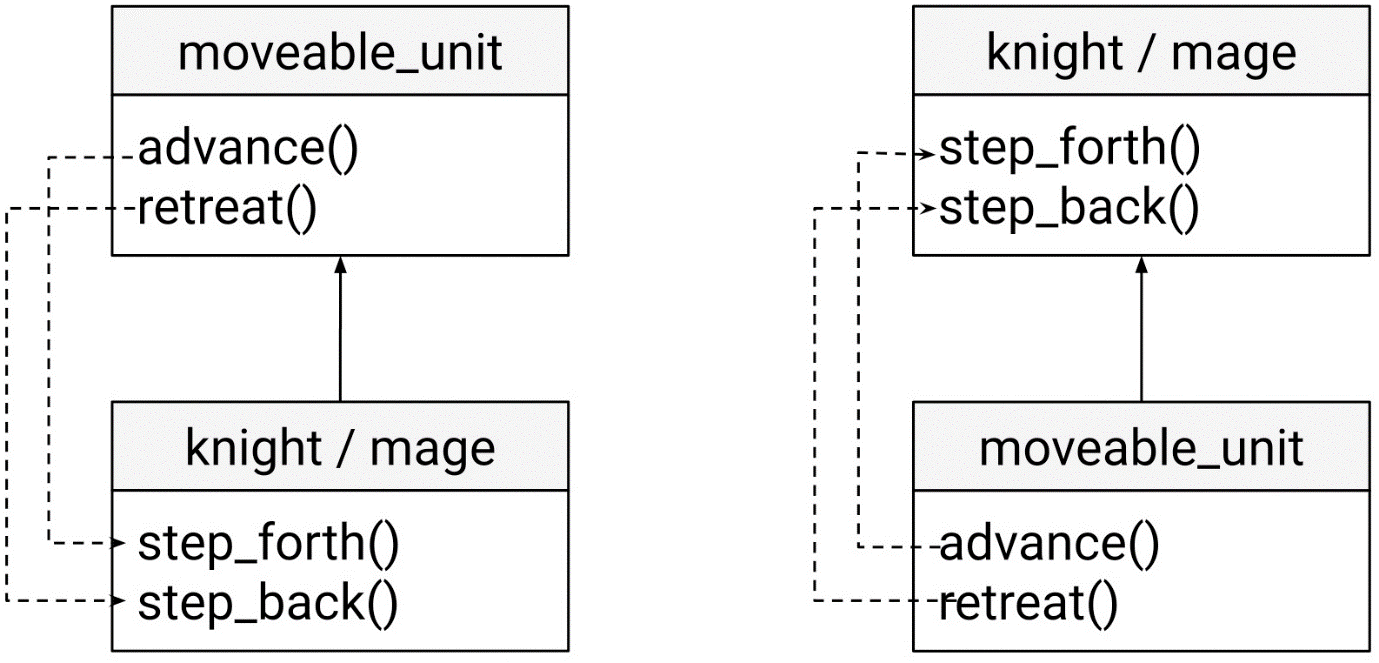
\includegraphics[width=0.7\textwidth]{content/3/chapter7/images/1.png}\\
Figure 7.1: Comparison of the CRTP and the mixins patterns
\end{center}

We can combine the static polymorphism achieved with mixins with dynamic polymorphism achieved with interfaces and virtual functions. We’ll demonstrate this with the help of an example concerning game units that fight. We had an earlier example when we discussed the CRTP, where the knight and mage classes had a member function called attack.

Let’s say we want to define multiple attacking styles. For instance, each game unit can use either an aggressive or a moderate attacking style. So that means four combinations: aggressive and moderate knights, and aggressive and moderate mages. On the other hand, both knights and mages could be lone warriors that are comfortable to fight alone, or are team players that always fight in a group with other units.

That means we could have lone aggressive knights and lone moderate knights as well as team player aggressive knights and team player moderate knights. The same applies to mages. As you can see, the number of combinations grows a lot and mixins are a good way to provide this added functionality without expanding the knight and mage classes. Finally, we want to be able to treat all these polymorphically at runtime. Let’s see how we can do this.

First, we can define aggressive and moderate fighting styles. These could be as simple as the following:

\begin{lstlisting}[style=styleCXX]
struct aggressive_style
{
	void fight()
	{
		std::cout << "attack! attack attack!\n";
	}
};

struct moderate_style
{
	void fight()
	{
		std::cout << "attack then defend\n";
	}
};
\end{lstlisting}

Next, we define mixins as the requirement of being able to fight alone or in a group. These classes are templates and are derived from their template argument:

\begin{lstlisting}[style=styleCXX]
template <typename T>
struct lone_warrior : T
{
	void fight()
	{
		std::cout << "fighting alone.";
		T::fight();
	}
};
template <typename T>
struct team_warrior : T
{
	void fight()
	{
		std::cout << "fighting with a team.";
		T::fight();
	}
};
\end{lstlisting}

Last, we need to define the knight and mage classes. These themselves will be mixins for the fighting styles. However, to be able to treat them polymorphically at runtime, we derive them from a base game\_unit class that contains a pure virtual method called attack that these classes implement:

\begin{lstlisting}[style=styleCXX]
struct game_unit
{
	virtual void attack() = 0;
	virtual ~game_unit() = default;
};

template <typename T>
struct knight : T, game_unit
{
	void attack()
	{
		std::cout << "draw sword.";
		T::fight();
	}
};

template <typename T>
struct mage : T, game_unit
{
	void attack()
	{
		std::cout << "spell magic curse.";
		T::fight();
	}
};
\end{lstlisting}

The knight and mage implementation of the attack member function makes use of the T::fight method. You have probably noticed that both the aggresive\_style and moderate\_style classes on one hand and the lone\_warrior and team\_warrior mixin classes on the other hand provide such a member function. This means we can do the following combinations:

\begin{lstlisting}[style=styleCXX]
std::vector<std::unique_ptr<game_unit>> units;

units.emplace_back(new knight<aggressive_style>());
units.emplace_back(new knight<moderate_style>());
units.emplace_back(new mage<aggressive_style>());
units.emplace_back(new mage<moderate_style>());
units.emplace_back(
	new knight<lone_warrior<aggressive_style>>());
units.emplace_back(
	new knight<lone_warrior<moderate_style>>());
units.emplace_back(
	new knight<team_warrior<aggressive_style>>());
units.emplace_back(
	new knight<team_warrior<moderate_style>>());
units.emplace_back(
	new mage<lone_warrior<aggressive_style>>());
units.emplace_back(
	new mage<lone_warrior<moderate_style>>());
units.emplace_back(
	new mage<team_warrior<aggressive_style>>());
units.emplace_back(
	new mage<team_warrior<moderate_style>>());

for (auto& u : units)
	u->attack();
\end{lstlisting}

In total, there are 12 combinations that we defined here. And this was all possible with only six classes. This shows how mixins help us add functionality while keeping the complexity of the code at a reduced level. If we run the code, we get the following output:

\begin{tcblisting}{commandshell={}}
draw sword.attack! attack attack!
draw sword.attack then defend
spell magic curse.attack! attack attack!
spell magic curse.attack then defend
draw sword.fighting alone.attack! attack attack!
draw sword.fighting alone.attack then defend
draw sword.fighting with a team.attack! attack attack!
draw sword.fighting with a team.attack then defend
spell magic curse.fighting alone.attack! attack attack!
spell magic curse.fighting alone.attack then defend
spell magic curse.fighting with a team.attack! attack attack!
spell magic curse.fighting with a team.attack then defend
\end{tcblisting}

We have looked here at two patterns, CRTP and mixins, that are both intended to add additional (common) functionality to other classes. However, although they look similar, they have opposite structures and should not be confused with one another. An alternative technique to leverage common functionalities from unrelated types is called type erasure, which we will discuss next.



































